\documentclass[../main.tex]{subfiles}
\begin{document}

\chapter{Conclusioni}

Lo studio di microrganismi tramite tecniche di microscopia a super-risoluzione è fondamentale per comprendere la loro struttura e i loro comportamenti. I batteri ESKAPE\cite{eskape} pongono oggi un serio rischio per la salute mondiale\cite{rice_2008} e una minaccia sempre crescente nel futuro.\cite{pipito_2025} Studiare questi batteri con le tecniche descritte in questa tesi può portare a una comprensione migliore dei loro fattori di virulenza e sviluppare nuovi farmaci che superano le loro resistenze per .

Effettuare questi studi con tecniche di microscopia come \acrshort{afm} e \acrshort{snom}, al posto di tecniche come la microscopia elettronica, ha il beneficio di non richiedere trattamenti speciali per i campioni, che invece potrebbero danneggiare o distruggere il campione. La microscopia \acrshort{afm} fornisce un profilo tridimensionale del campione, da cui si possono anche ottenere le sue proprietà viscoelastiche, mentre la microscopia \acrshort{snom} fornisce informazioni sulle sue proprietà ottiche, come l'indice di rifrazione.

Queste due tecniche di microscopia funzionano senza aver bisogno di ambienti particolari, come una camera a vuoto o criogenica, rendendole un buono strumento per lo studio di macromolecole e organismi viventi. inoltre, queste tecniche possono essere combinate nello stesso microscopio per ottenere più informazioni correlate della stessa scansione.

\section{Analisi correlativa}
La microscopia \acrshort{ssnom} ha suscitato interesse negli ultimi anni, ma il suo impiego nella \gls{microbiologia} è rimasto limitato, soprattutto per le difficoltà nell'interpretare i dati a causa della scarsa disponibilità dei dati. Come accennato in precedenza, un microscopio può offrire più tecniche di microscopia per studiare più proprietà dello stesso materiale nello stesso momento, per questo recenti studi hanno accoppiato un sistema di microscopia \acrshort{ssnom} ad altri sistemi per avere un contesto noto per analizzare i dati provenienti dal campo vicino, come la microscopia \acrfull{afm} o \acrshort{clsm}.\cite{stanciu_2017}\\

\begin{figure}[h]
	\centering
	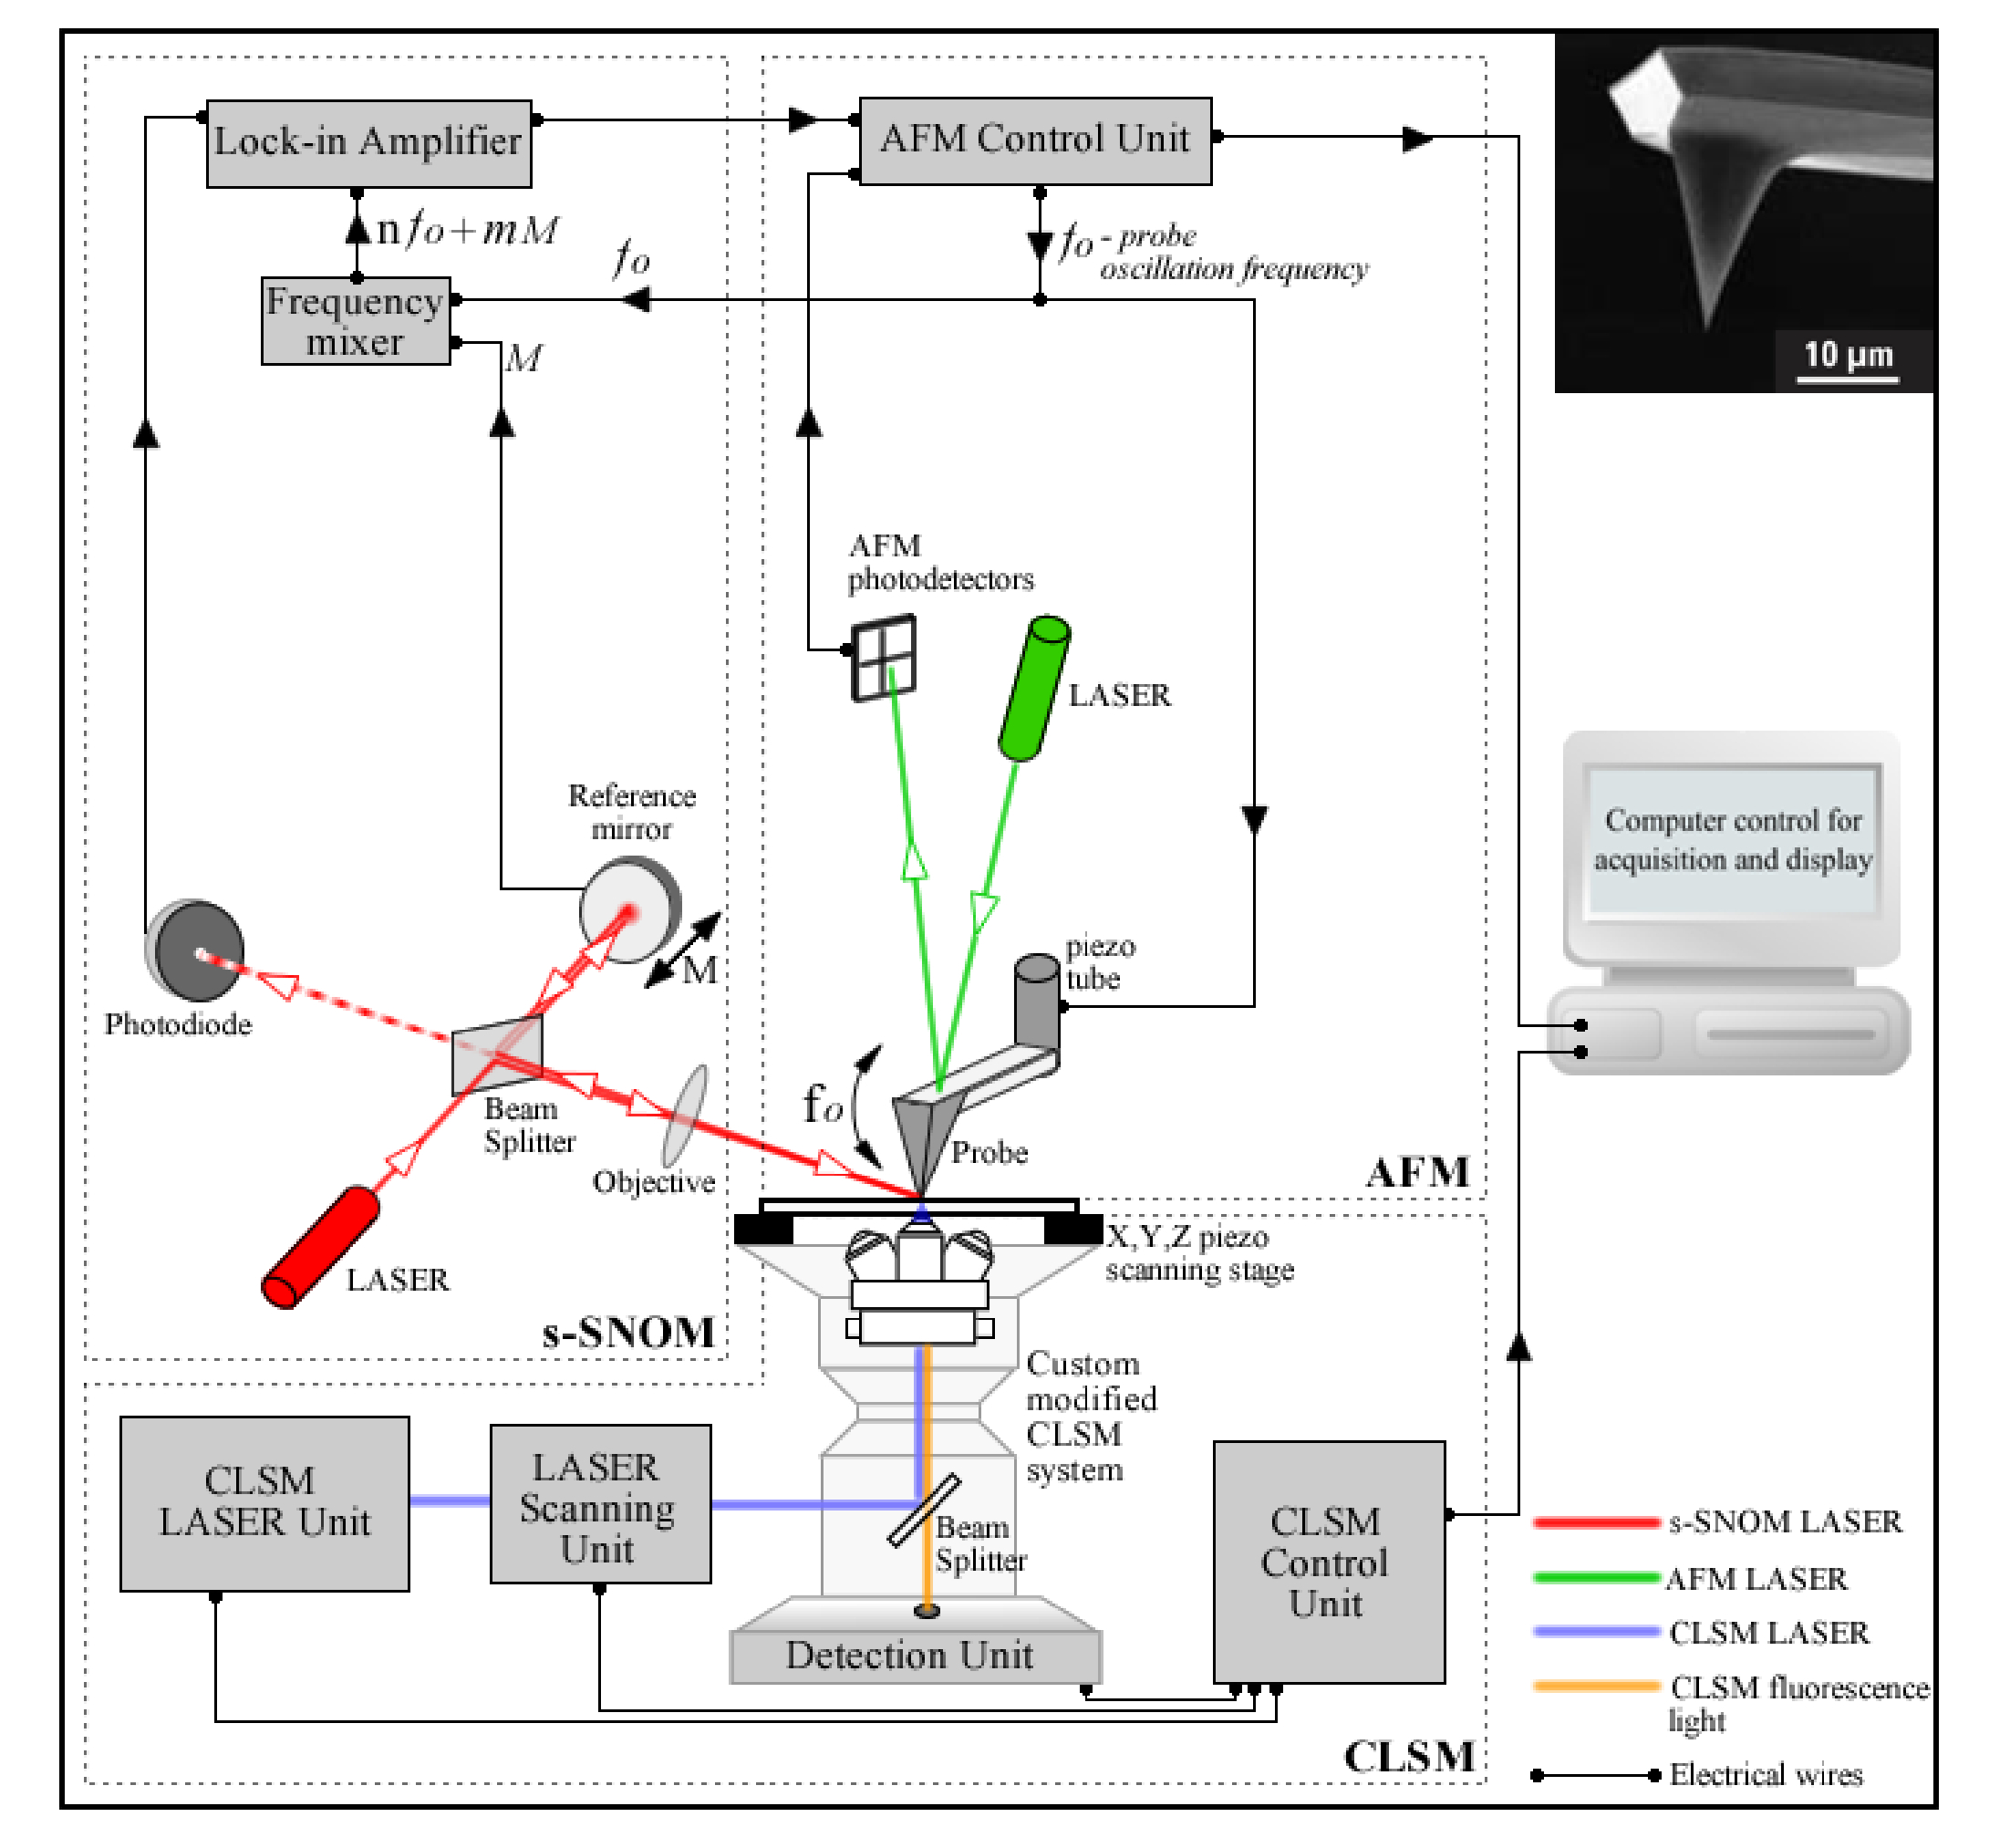
\includegraphics[keepaspectratio, height=\linewidth]{images/multimodal_system.jpg}
	\caption[Sistema multimodale per l'acquisizione di immagini correlative]{
		Sistema multimodale per l'acquisizione di immagini correlative \cite{stanciu_2017}}
	\label{fig:multimodal_system}
\end{figure}

\section{Rumore}

Uno dei problemi nel comprendere ed automatizzare l'elaborazione di queste immagini è la quantità di rumore al quale sono affette. Uno dei parametri che più influenza la quantità di rumore nelle immagini è il tempo di integrazione per pixel della scansione: più è alto questo parametro, più il rumore sarà attenuato. Il problema nel fare ciò sta nel fatto che un tempo di integrazione alto aumenta il rischio di dislocare il campione e aumenta il tempo di scansione, infatti per le immagini del dataset di SSNOMBACTER è stato usato un tempo di integrazione di $3$ ms, che equivale a un tempo di scansione di quasi $5$ minuti.

Usare delle tecniche di riduzione del rumore permette di aumentare i dettagli mantenendo un tempo di integrazione basso e riducendo il tempo richiesto per l'acquisizione. Dalle valutazioni esposte in questa tesi si evince come, per immagini in cui il rumore di tipo impulsivo sia elevato è consigliato usare un fi
ltro mediana al costo di una leggera sfocatura dei dettagli, mentre è consigliato usare un filtro a media non locale in immagini con poco rumore impulsivo per rimuovere in modo efficace il rumore gaussiano mantenendo intatti i dettagli del campione.

\section{Sviluppi futuri}

La scarsa disponibilità di dati, meno di 100 scansioni, non permette l'uso di tecniche di deep learning per classificare la qualità delle immagini o per ridurre il rumore in modo affidabile senza incorporare dati esterni, come dei rank o punteggi soggettivi come il \acrshort{mos} (\acrlong{mos}), visto che per poter usare queste tecniche più moderne è richiesta una grande quantità di dati per l'apprendimento.\cite{lecun_2015,litjens_2017,bosse_2018} Una soluzione sarebbe quella di acquisire più scansioni ma, data la grande quantità di tempo richiesta per effettuarle, si può prendere in considerazione anche l'uso di AI generativa, come un modello di diffusione, per estendere il dataset con immagini sintetiche partendo da quelle presenti.\cite{ho_2020}

Questo studio può essere esteso ad altri tipi di filtri basati sulla mediana per valutare la loro efficacia nel rimuovere il rumore impulsivo su questo tipo di immagini. Di seguito è presentata una lista di alcuni possibili filtri:

\begin{itemize}
	\itemsep 0em
	\item \acrfull{mf}\cite{gallagher_1981} --- il filtro usato in questa tesi
	\item \acrfull{wmf}\cite{zhang_2009}
	\item \acrfull{cwmf}\cite{ko_1991}
	\item \acrfull{rwmf}\cite{kumar_2007}
	\item \acrfull{amf}\cite{chen_2001}
	\item \acrfull{asmf}\cite{khryashchev_2005}
	\item \acrfull{psmf}\cite{wang_1999}
	\item \acrfull{tsmf}\cite{chen_1999}
\end{itemize}

\section{Ulteriori elaborazioni}

Le immagini ottenute dall'applicazione delle tecniche di riduzione del rumore possono essere usate in applicazioni di visione artificiale per compiti come la conta delle cellule nell'immagine, lo studio delle loro caratteristiche morfologiche, come la rugosità della parete, la sua conformazione e come si dispongono gruppi di cellule. Un altro campo di interesse molto importante è la classificazione delle specie partendo dalle immagini o lo studio della mobilità dei batteri con flagelli e il loro riconoscimento.

\subsection{Segmentazione}

In questa tesi viene portato come esempio un processo di instance segmentation automatizzato.\cite{hafiz_2020} Per prima cosa sono state create manualmente delle regioni di interesse corrispondenti ai batteri sulle immagini, in questo caso tutte della stessa classe. Poi è stato fatto il fine-tuning di un modello \acrshort{yolo} (\acrlong{yolo}) sulla maggior parte delle immagini mentre il restante 20\% è stato usato per la validazione dei risultati. Per fare ciò è stato usato il modello \texttt{yolo11m-seg} di Ultralytics\cite{ultralytics_2023}, licenziato secondo la licenza AGPL-3.0. Il modello ha dato buoni risultati, con una precisione dell'80.35\%, un recupero dell'82.72\%, una mAP50 dell82.19\% e una mAP50-95 del 62.65\%.

\begin{figure}[h]
	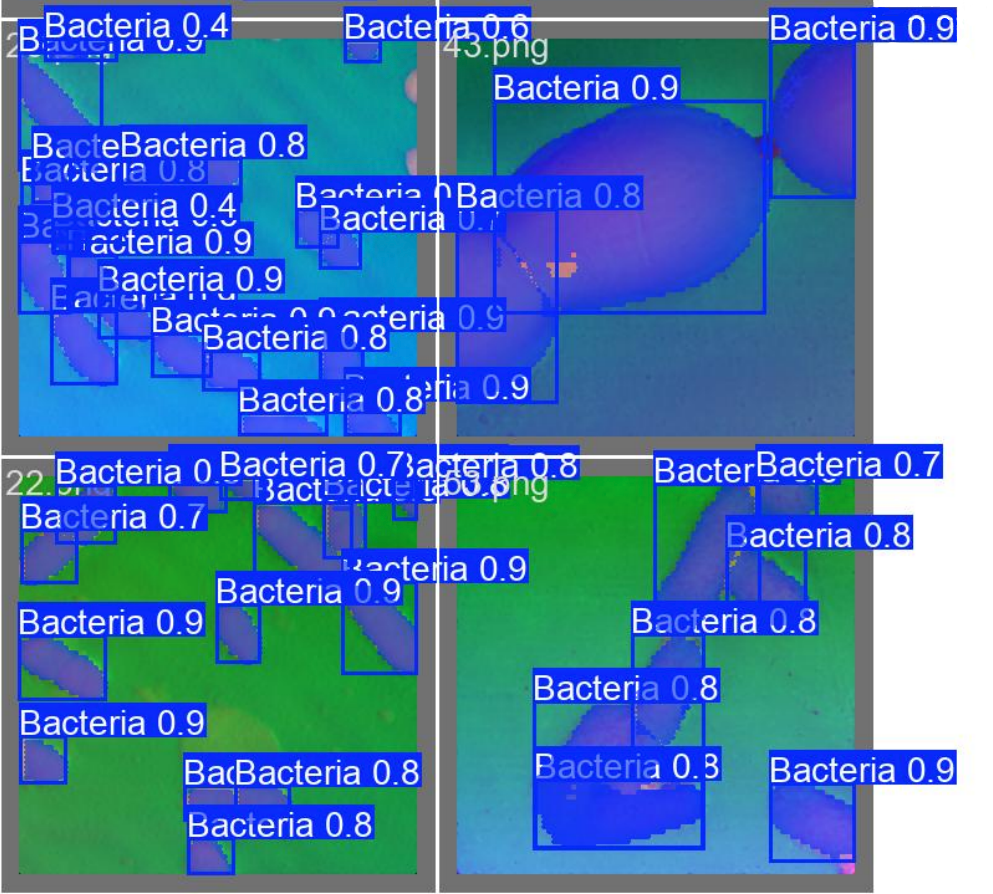
\includegraphics[keepaspectratio,width=\linewidth]{images/seg_val.png}
	\caption{Alcuni risultati della segmentazione}
\end{figure}

\end{document}